\documentclass[letter,twocolumn]{revtex4}
\usepackage[utf8]{inputenc}

\usepackage{epsfig}
\usepackage{graphicx}
\usepackage{tikz}
\usetikzlibrary{shapes.geometric, arrows}
\graphicspath{ {images/} }
\usepackage{listings}
\usepackage{color}

\usepackage{xcolor}

\definecolor{codegreen}{rgb}{0,0.6,0}
\definecolor{codegray}{rgb}{0.5,0.5,0.5}
\definecolor{codepurple}{rgb}{0.58,0,0.82}
\definecolor{backcolour}{rgb}{0.95,0.95,0.92}

\lstdefinestyle{mystyle}{
    backgroundcolor=\color{backcolour},   
    commentstyle=\color{codegreen},
    keywordstyle=\color{magenta},
    numberstyle=\tiny\color{codegray},
    stringstyle=\color{codepurple},
    basicstyle=\ttfamily\footnotesize,
    breakatwhitespace=false,         
    breaklines=true,                 
    captionpos=b,                    
    keepspaces=true,                 
    numbers=left,                    
    numbersep=5pt,                  
    showspaces=false,                
    showstringspaces=false,
    showtabs=false,                  
    tabsize=2
}

\lstset{style=mystyle}


\begin{document}

\title{Práctica 1: Minipunto de Venta}
\author{Archundia Bazán Aarón Antonio, Guerrero Velez Eliseo Milton, Hernández Vázquez Cesar Arturo}
\affiliation{Unidad Profesional Interdisciplinaria en Ingenier\'{\i}a y Tecnolog\'{\i}as Avanzadas del I.P.N.\\ Ingeniería Biónica,Programación Orientada a Objetos}

\date{26 de octubre de 2020}
\maketitle


\section{Planteamiento del problema}


        El problema consiste en crear un sistema de punto de venta que le permita al usuario o al empleado que desee generar tickets con los productos disponibles. Hay cinco productos disponibles en la tienda con cinco precios diferentes enumerados en la tabla I.I:
\begin{center}
        \begin{tabular}{|c|c|c}
                \hline
                Producto  & Precio \\
                \hline
                Producto 1 & \$2.98 \\
                \hline
                Producto 2 & \$4.50 \\
                \hline
                Producto 3  & \$9.98 \\
                \hline
                Producto 4 & \$4.49  \\
                \hline
                Producto 5  & \$6.87 \\
                \hline
        
        \end{tabular}
\caption{Tabla I.I. Productos disponibles con sus precios }    
\end{center}
\section{Propuesta de Solución}
    Para solucionar el problema se propuso  encontrar la sumatoria total de artículos comprados,  haciendo el producto de cada articulo por su cantidad vendida.
    
                 \begin{center}
                        $VentaT = \sum (Precioproducto*Cantidadvendida)$
                 \end{center}  
        
                 Como únicamente son cinco productos la sumatoria se haría del producto1 hasta el producto5
        
                \begin{center}
                       $VentaT = \sum\limits_{N_p=1}^{N_p=5} (Precioproducto*cantidadvendida)$
                \end{center}
    
    Esto se ejecutará  cíclicamente dependiendo de cuantos productos requiera comprar el usuario  si el usuario únicamente quiere un producto,  la sentencia de control do-while permitirá que el usuario ejecute una vez y termine pero también si quiere tomar otro producto continuará hasta que termine de escoger y diga que ya no quiere continuar comprando. Finalmente se le imprimirá un ticket de compra con el fin de que vea cuales fueron sus gastos parciales y totales. 
    \\\\\\\\\\\\


\section{Análisis y diseño}

\subsection{Diagrama de flujo}
\begin{figure}[ht]
         \renewcommand\figurename{Fig.}
         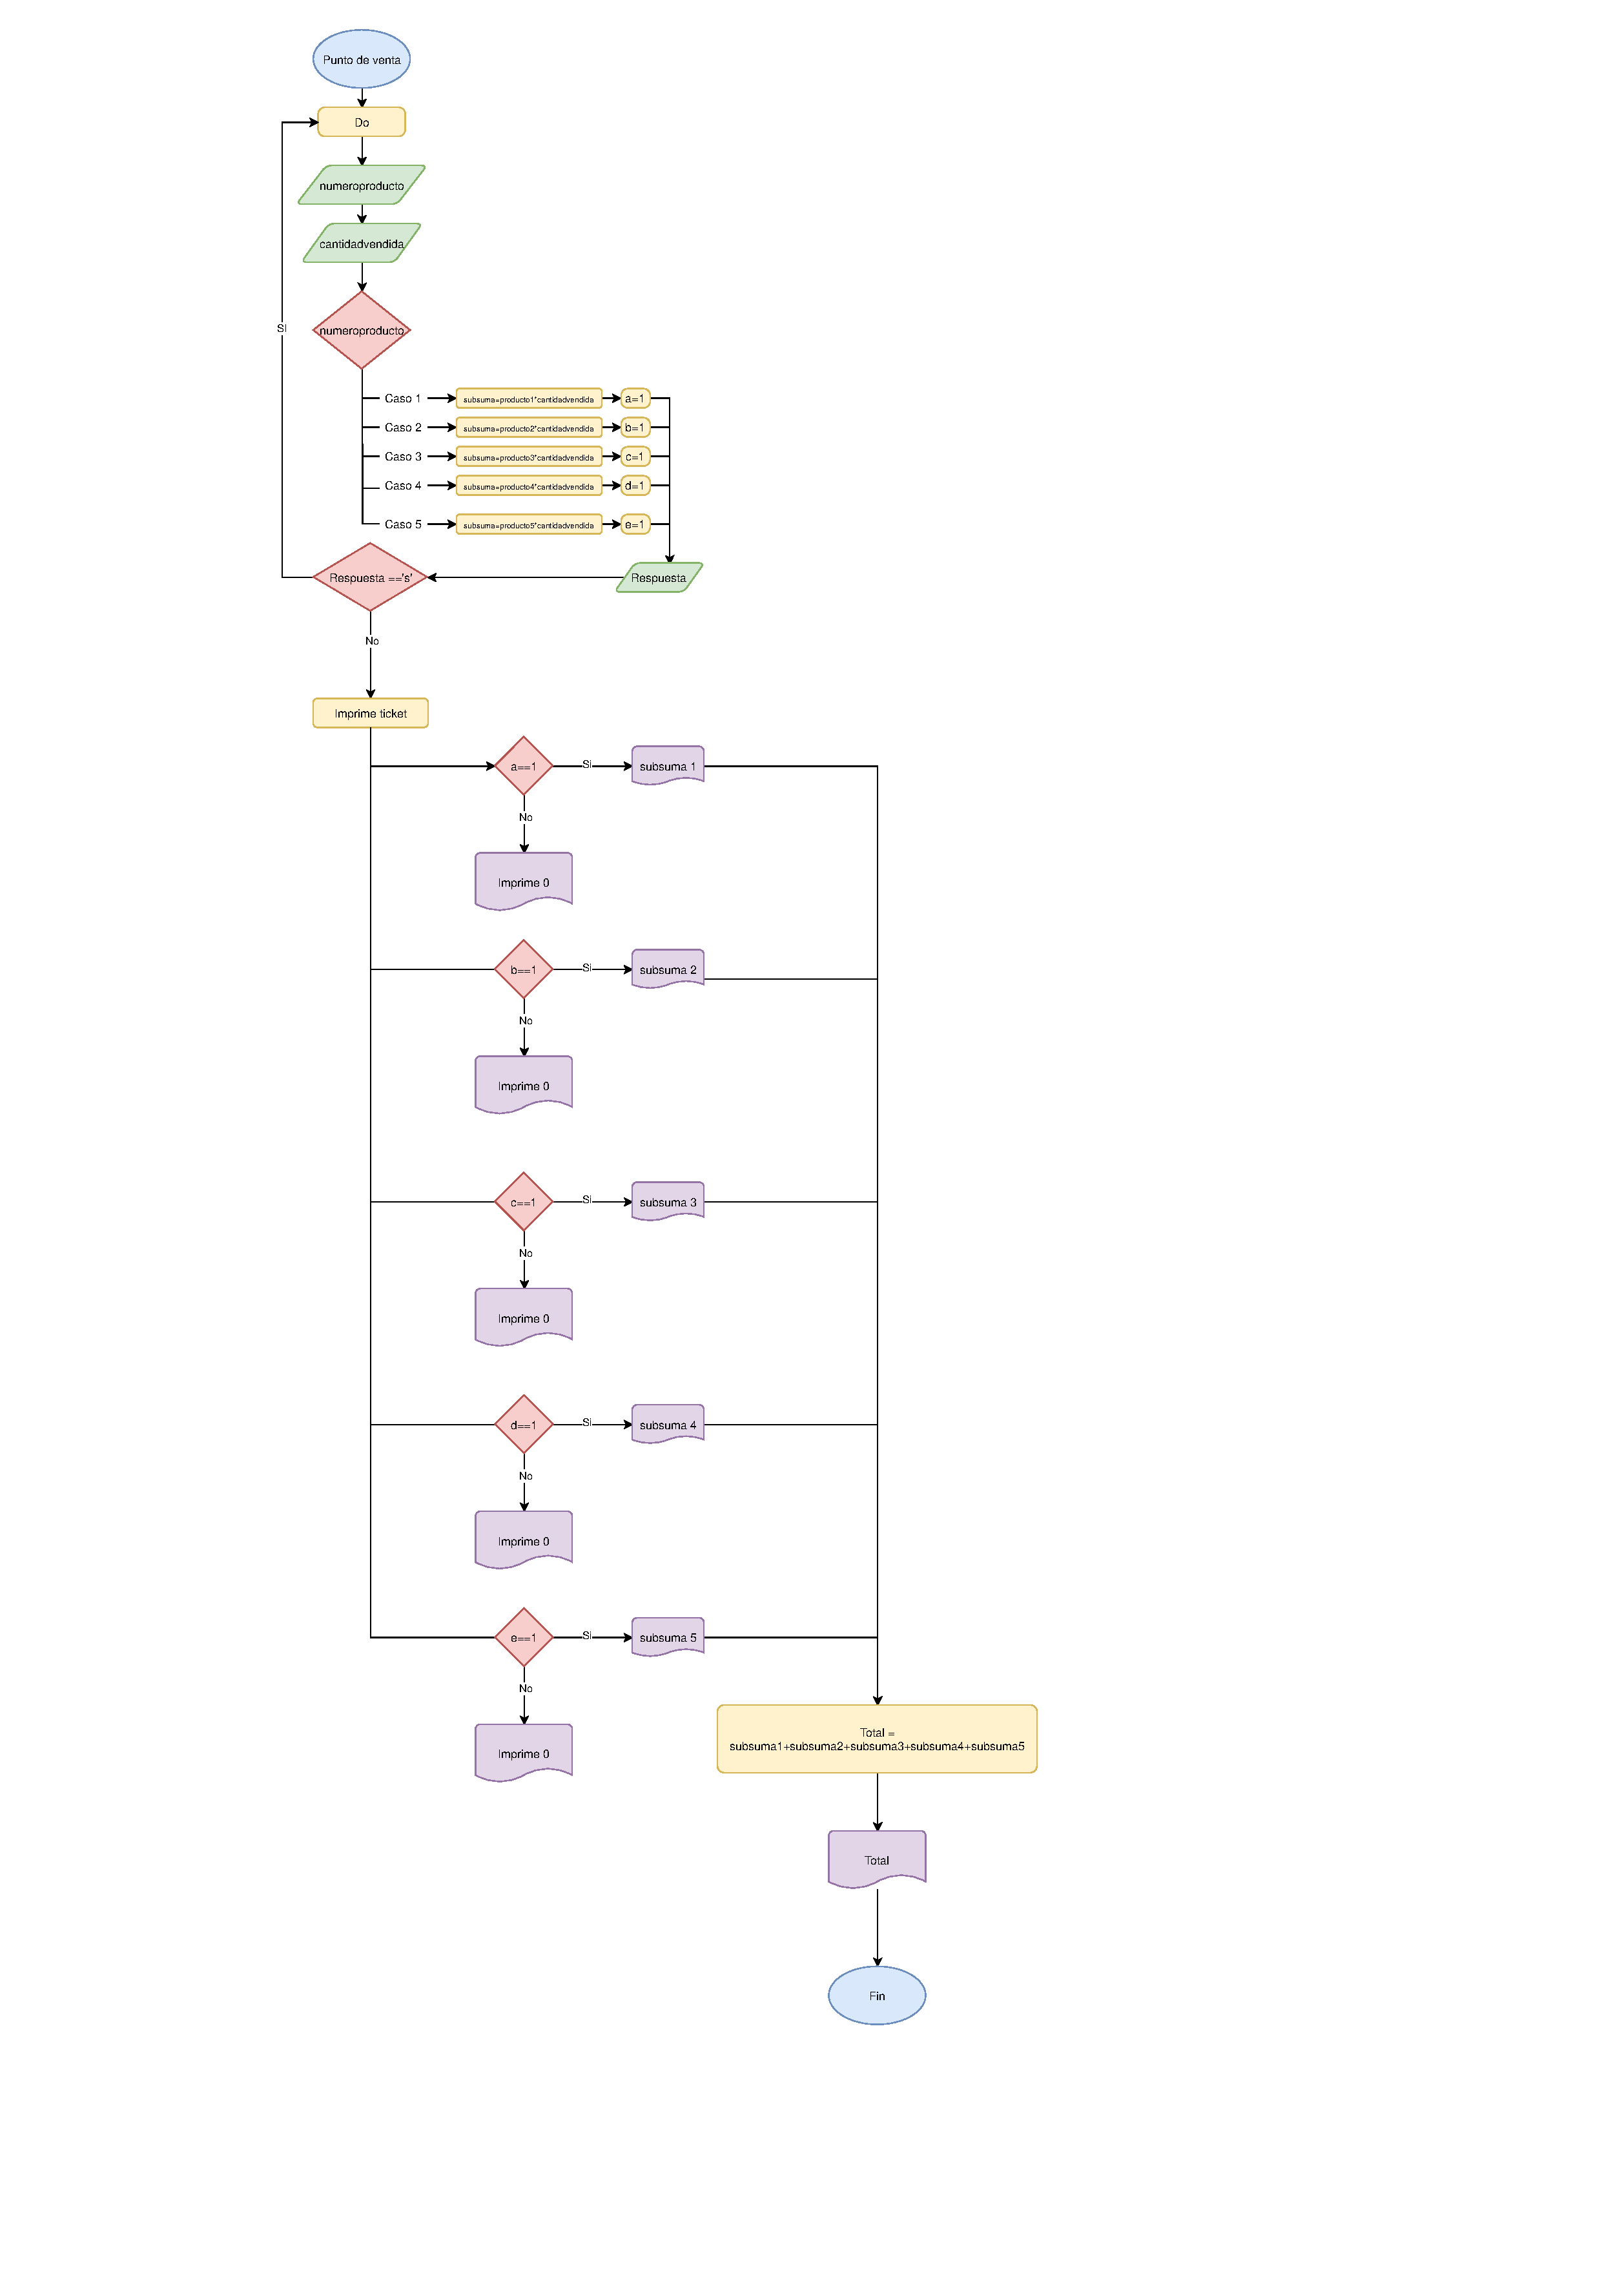
\includegraphics[scale=0.25]{Images/Diagrama.eps}
         \caption{Diagrama de flujo, Minipunto de venta}
\end{figure}

\clearpage

\section{Implementación y pruebas}
    Se utilizó la plataforma GitHub para el control de versiones de nuestro minipunto de venta donde se hicieron los cambios pertinentes con el fin de trabajar en equipo en linea.
    
    
    \begin{figure}[ht]
         \renewcommand\figurename{Fig.}
         \includegraphics[scale=0.3]{Images/Captura de pantalla (213).png}
         \caption{Cambios hechos por integrante}
    \end{figure}
    
    
    \begin{figure}[ht]
             \renewcommand\figurename{Fig.}
             \includegraphics[scale=0.2]{Images/Captura de pantalla (214).png}
             \caption{Cambios con el tiempo (Rojo, código borrado,Verde, código actual)}
    \end{figure}
\subsection{Caso I.}
Cuando solo se requiere comprar un solo producto, solo se hará la multiplicación entre la cantidad de piezas y el precio unitario.     
\begin{center}
\begin{large}
        $ VentaT =  precioproducto * cantidadvendida $
\end{large}
\end{center}
        
    \begin{figure}[ht]
             \renewcommand\figurename{Fig.}
             \includegraphics[scale=0.5]{Images/Paso1.PNG}
             \caption{Paso 1: Elegir producto}
    \end{figure}
   
   
     \begin{figure}[ht]
             \renewcommand\figurename{Fig.}
             \includegraphics[scale=0.5]{Images/Paso2.PNG}
             \caption{Paso 2: Elegir la cantidad de piezas }
     \end{figure}  
     
     
     \begin{figure}[ht]
             \renewcommand\figurename{Fig.}
             \includegraphics[scale=0.5]{Images/Paso3.PNG}
             \caption{Paso 3: Se despliega el Ticket de compra con el precio de los productos adquiridos}
     \end{figure}  

\clearpage
\subsection{Caso II.}
Cuando se van a comprar más de un articulo 

\clearpage
        
\clearpage




\section{Código fuente comentado}

\lstinputlisting[language=C++]{Minishop.cpp}


\section{Conclusiones}





\end{document}